\usetikzlibrary{fit, calc, positioning, arrows.meta}


\chapter{Calcolo delle componenti connesse di un grafo non orientato}

\section{Definizione delle Componenti Connesse}
Una cc di un grafo non orientato $G$ è un sottografo massimale nel quale $\forall i,j$ vertici in cc $j$ è raggiungibile da $i$ ossia è una classe di equivalenza della relazione "raggiungibile"

\section{Definizione del problema}
\subsection{Istanza}
Un sottografo nel quale per ogni coppia di vertici c'è un cammino

\begin{figure}[htbp]
\centering
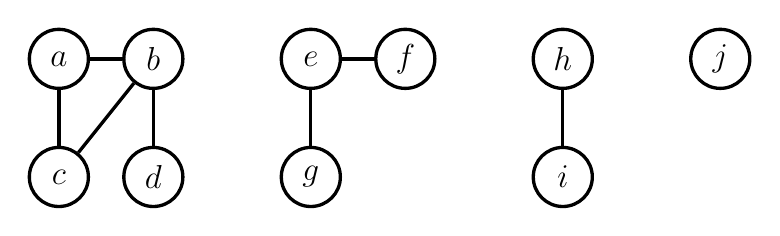
\begin{tikzpicture}[
    vnode/.style={circle, draw=black, very thick, minimum size=7.5mm, inner sep=0pt, font=\large},
    edge/.style={very thick}
]

    % --- 1° Componente Connessa ---
    \node[vnode] (a) at (0, 1.5) {$a$};
    \node[vnode] (b) at (1.2, 1.5) {$b$};
    \node[vnode] (c) at (0, 0) {$c$};
    \node[vnode] (d) at (1.2, 0) {$d$};
    
    \draw[edge] (a) -- (b);
    \draw[edge] (a) -- (c);
    \draw[edge] (b) -- (c);
    \draw[edge] (b) -- (d);

    % --- 2° Componente Connessa ---
    \node[vnode] (e) at (3.2, 1.5) {$e$};
    \node[vnode] (f) at (4.4, 1.5) {$f$};
    \node[vnode] (g) at (3.2, 0) {$g$};
    
    \draw[edge] (e) -- (f);
    \draw[edge] (e) -- (g);

    % --- 3° Componente Connessa ---
    \node[vnode] (h) at (6.4, 1.5) {$h$};
    \node[vnode] (i) at (6.4, 0) {$i$};
    
    \draw[edge] (h) -- (i);

    % --- 4° Componente Connessa ---
    \node[vnode] (j) at (8.4, 1.5) {$j$};

\end{tikzpicture}
\end{figure}

\subsection{Obiettivo}
Calcolare le cc di un grafo.

Si hanno 2 opzioni per fare ciò

\subsection{Soluzione mediante modifica dell'algoritmo DFS}
\begin{minipage}{0.45\textwidth}
    \begin{algorithmic}
        \Procedure{CC-DFS}{$G$}
            \For{ogni $v \in V$}
                \State $v.col=WHITE$
            \EndFor

            \State $k=0$

            \For{ogni $v \in V$}
                \If{$v.col=WHITE$}
                    \State $k=k+1$
                    \State \Call{CC-DFS-VISIT}{$v$}
                \EndIf
            \EndFor
        \EndProcedure
    \end{algorithmic}
\end{minipage}
\hfill
\begin{minipage}{0.45\textwidth}
    \begin{algorithmic}
        \Procedure{CC-DFS-VISIT}{$v$}
            \State $\boxed{v.cc = k}$
            \State $v.col = \text{GRAY}$
            \State $\vdots$
            \For{ogni $v \dots$}
                \State $\vdots$
                \State \Call{CC-DFS-VISIT}{$v$}
            \EndFor
        \EndProcedure
    \end{algorithmic}
\end{minipage}

\section{Soluzione sfruttando le strutture dati per insiemi disgiunti con $\mathbf{X=V}$}

Si parte dalla collezione $\{\{v_1\},\{v_2\}, \dots, \{v_n\}\}$ e si vuole arrivare a $\{C^1, \dots, C^n\}$ ove $C^i$ contiene i vertici della cc $i$

\begin{figure}[htbp]
\centering
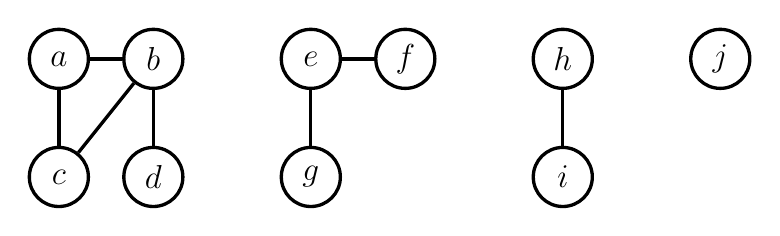
\begin{tikzpicture}[
    vnode/.style={circle, draw=black, very thick, minimum size=7.5mm, inner sep=0pt, font=\large},
    edge/.style={very thick}
]

    % --- 1° Componente Connessa ---
    \node[vnode] (a) at (0, 1.5) {$a$};
    \node[vnode] (b) at (1.2, 1.5) {$b$};
    \node[vnode] (c) at (0, 0) {$c$};
    \node[vnode] (d) at (1.2, 0) {$d$};
    
    \draw[edge] (a) -- (b);
    \draw[edge] (a) -- (c);
    \draw[edge] (b) -- (c);
    \draw[edge] (b) -- (d);

    % --- 2° Componente Connessa ---
    \node[vnode] (e) at (3.2, 1.5) {$e$};
    \node[vnode] (f) at (4.4, 1.5) {$f$};
    \node[vnode] (g) at (3.2, 0) {$g$};
    
    \draw[edge] (e) -- (f);
    \draw[edge] (e) -- (g);

    % --- 3° Componente Connessa ---
    \node[vnode] (h) at (6.4, 1.5) {$h$};
    \node[vnode] (i) at (6.4, 0) {$i$};
    
    \draw[edge] (h) -- (i);

    % --- 4° Componente Connessa ---
    \node[vnode] (j) at (8.4, 1.5) {$j$};

\end{tikzpicture}
\end{figure}

\vspace{0.5cm}

\noindent Nell'esempio si parte da
\[
\Bigl\{ \{a\}, \{b\}, \{c\}, \{d\}, \{e\}, \{f\}, \{g\}, \{h\}, \{i\}, \{j\} \Bigr\}
\]
e si vuole arrivare a
\[
\Bigl\{ \{a, b, c, d\}, \{e, f, g\}, \{h, i\}, \{j\} \Bigr\}
\]
\normalsize

Si uniscono due insiemi disgiunti se $\exists u,v \in V :$
\begin{itemize}
    \item $u \in$ primo insieme
    \item $v \in$ secondo insieme
    \item $(u,v) \in E$
\end{itemize}

si considerano tutti gli archi

{
    \large

    \begin{figure}[htbp]
        \centering

        % --- PARTE 1: Disegno dei grafi (Stato finale) ---
        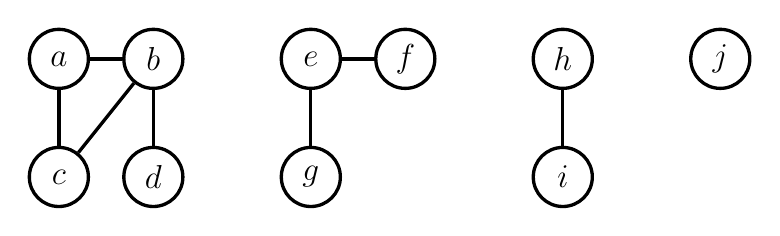
\begin{tikzpicture}[
            vnode/.style={circle, draw=black, very thick, minimum size=7.5mm, inner sep=0pt, font=\large},
            edge/.style={very thick}
        ]

            % Componente 1
            \node[vnode] (a) at (0, 1.5) {$a$};
            \node[vnode] (b) at (1.2, 1.5) {$b$};
            \node[vnode] (c) at (0, 0) {$c$};
            \node[vnode] (d) at (1.2, 0) {$d$};
            \draw[edge] (a) -- (b);
            \draw[edge] (a) -- (c);
            \draw[edge] (b) -- (c);
            \draw[edge] (b) -- (d);

            % Componente 2
            \node[vnode] (e) at (3.2, 1.5) {$e$};
            \node[vnode] (f) at (4.4, 1.5) {$f$};
            \node[vnode] (g) at (3.2, 0) {$g$};
            \draw[edge] (e) -- (f);
            \draw[edge] (e) -- (g);

            % Componente 3
            \node[vnode] (h) at (6.4, 1.5) {$h$};
            \node[vnode] (i) at (6.4, 0) {$i$};
            \draw[edge] (h) -- (i);

            % Componente 4
            \node[vnode] (j) at (8.4, 1.5) {$j$};

        \end{tikzpicture}

        % --- PARTE 2: Tabella di tracciamento operazioni UNION ---
        % Definisco un comando inline per creare la freccia curva con il testo
        \newcommand{\unionarrow}[1]{%
            \begin{tikzpicture}[baseline=-0.7ex]
                \draw[-{Stealth[length=2.5mm]}, thick] (-0.3, 0.5) to[out=0, in=90] (-0.05, 0.25) to[out=-90, in=180] (0.2, 0) node[right, inner sep=2pt, font=\normalsize\bfseries] {UNION (#1)};
            \end{tikzpicture}%
        }

        \[
        \renewcommand{\arraystretch}{1.5} % Aumenta l'altezza delle righe per far respirare le frecce
        \begin{array}{r|l@{\hspace{0.5cm}}l}
            & \{a\} \ \{b\} \ \{c\} \ \{d\} \ \{e\} \ \{f\} \ \{g\} \ \{h\} \ \{i\} \ \{j\} & \\
        \hline
        (b,d) & \{a\} \ \{b,d\} \ \{c\} \ \{e\} \ \{f\} \ \{g\} \ \{h\} \ \{i\} \ \{j\} & \unionarrow{b,d} \\
        (e,g) & \{a\} \ \{b,d\} \ \{c\} \ \{e,g\} \ \{f\} \ \{h\} \ \{i\} \ \{j\}       & \unionarrow{e,g} \\
        (a,c) & \{a,c\} \ \{b,d\} \ \{e,g\} \ \{f\} \ \{h\} \ \{i\} \ \{j\}             & \unionarrow{a,c} \\
        (h,i) & \{a,c\} \ \{b,d\} \ \{e,g\} \ \{f\} \ \{h,i\} \ \{j\}                   & \unionarrow{h,i} \\
        (a,b) & \{a,b,c,d\} \ \{e,g\} \ \{f\} \ \{h,i\} \ \{j\}                         & \unionarrow{a,b} \\
        (e,f) & \{a,b,c,d\} \ \{e,f,g\} \ \{h,i\} \ \{j\}                               & \unionarrow{e,f} \\
        (b,c) & \hspace{1cm} '' \hspace{1.3cm} '' \hspace{1.1cm} '' \hspace{1.1cm} ''   & \quad \textbf{NO UNION} \\
        \end{array}
        \]

    \end{figure}
}


\begin{minipage}{0.45\textwidth}
    \begin{algorithmic}
    \Procedure{CONNECTED-COMPONENT}{$G$}
        \State $G=(V,E)$
        \State $n = |V|$

        \For{$i=1$ to $n$}
            \State \Call{MAKE-SET}{$v_i$}
        \EndFor

        \For{ogni $(u,v) \in E$}
            \If{\Call{FIND-SET}{$u$} $\not = $ \Call{FIND-SET}{$v$}}
                \State \Call{UNION}{$u,v$}
            \EndIf
        \EndFor
    \EndProcedure
\end{algorithmic}
\end{minipage}
\hfill
\begin{minipage}{0.45\textwidth}
    \begin{algorithmic}
        \Procedure{SAME-CC}{$u,v$}
            \If{\Call{FIND-SET}{$u$} = \Call{FIND-SET}{$v$}}
                \State \Return $true$

                \Else
                    \State \Return $false$
            \EndIf
        \EndProcedure
    \end{algorithmic}
\end{minipage}